

\section{Modellierung}

Die Software ist stark modularisiert und dom\"anenorientiert aufgebaut.
Wichtige Aspekte, die zu dieser Entscheidung gef\"uhrt haben, sind unter anderem,
dass die Software sp\"ater einfach und schnell erweitbar, \"anderbar und partiell wiederverwendbar sein soll.
Die Modularisierung erfolgt nach Funktionen und Teilaufgaben innerhalb einer Funktion.
ApoCo wird mittels verschiedener Architekturen realisiert.
Zun\"achst ist die grobe Struktur der Android-Anwendung als \emph{Model-View-Controller (MVC)} modelliert.
Die einzelnen Schichten Model, View und Controller der Android-Anwendung sind wie in der Abbildung 4.1 aufgeteilt.\\

\begin{figure}[h]
  \centering
  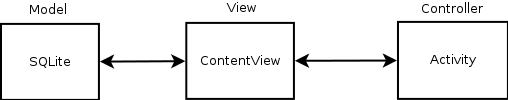
\includegraphics[scale=0.7]{diagramme/kapitel4/MVC.png}
  \caption{MVC-Architektur der ApoCo-Anwendung}
 
\end{figure}

\begin{itemize}
 \item Model: Die Model-Schicht ist die interne Datenbank der ApoCo-Anwendung.
 Als Datenbank nutzt Android SQLite.
 Dabei ist die Datenbank als eine Datei umgesetzt.
 Diese ist auf dem Dateisystem in Ordnern der ApoCo-Anwendung hinterlegt.
 Die Anfragen und Statements werden hier genauso verwendet wie das zum Beispiel der Fall bei MySQL oder Oracle Datenbanken ist.
 
 \item View: Die View-Schicht wird durch die \emph{Views} einer Android-Activity repr\"asentiert.
 Eine solche View wird in den meisten F\"allen in einer XML-Datei beschrieben.
 Diese Datei enth\"alt die Struktur einer View, welche dem Benutzer anschlie\ss{}end auf dem Bildschirm pr\"asentiert wird.
  
 \item Controller: Die Controller-Schicht wird durch die Anwendungslogik in den Activities umgesetzt.
 Hier wird die Interaktion des Patienten mit ApoCo abgefangen und die Ausgaben f\"ur den Bildschirm gesteuert.
\end{itemize}


Wird das gesamte Projekt betrachtet, handelt es sich dabei um eine Client-Server-Architektur.
In der Abbildung 4.2 wird die Aufteilung der einzelnen Software-Komponenten der Client-Server-Architektur dargestellt.\\

\begin{figure}[h]
  \centering
  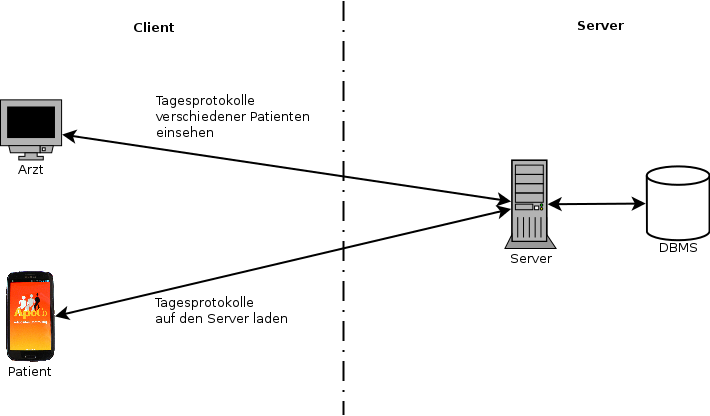
\includegraphics[scale=0.5]{diagramme/kapitel4/client_server.png}
  \caption{Client-Server-Architektur des gesamten Projekts}
  
\end{figure}

ApoCo ist der Teil der gesamten Software, welcher sich um das Aufzeichnen von Tagesprotokollen k\"ummert.
Um die Daten auswerten zu k\"onnen, benutzt der Arzt eine Webanwendung.
Dabei werden die Tagesprotokolle von der Datenbank geladen und im Webbrowser des Arztes angezeigt.\\
 
